Задача описания поведения некоторой системы во времени сводится к выяснению связи
межу~<<сигналом>>, подаваемым на <<вход>> системы (обозначим его как $f(t)$),
и её реакцией на <<выходе>> ($g(t)$):
\[
f(t)\to\fbox{?} \to g(t).
\]
В этой главе мы рассмотрим \important{спектральный} метод решения данной задачи применительно
к \important{линейным} системам.

\begin{wrapfigure}[10]{o}{0.3\textwidth}
% \psfragfig[width=0.25\textwidth]{Images/Chapter_6/1}{%
%     \psfrag{f}[cc]{$f(t)$}
%     \psfrag{g}[cl]{$g(t)$}
%     \psfrag{r}[ct]{$R$}
%     \psfrag{c}[cr]{$C$}
%     \psfrag{l}[cb]{$L$}}
\centering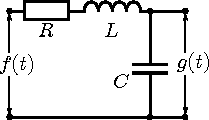
\includegraphics[scale=0.9]{Chapter_6/v6-RLC}
    \caption{Входной и выходной сигналы в $RLC$-контуре}
    \figmark{RLC circuit}
\end{wrapfigure}

Прежде, чем излагать теорию в общем виде, рассмотрим конкретный пример.
Пусть на вход колебательного $RLC$-кон\-ту\-ра подано некоторое
напряжение $U_{вх}=f(t)$. Будем снимать напряжение с конденсатора:
$U_{вых}=U_C = g(t)$. Попробуем выяснить, как связаны~$f(t)$ и~$g(t)$.

Ответ хорошо известен, если $f(t)$~--- гармоническая функция некоторой частоты~$\omega$.
Пусть в комплексном представлении $f(t)=c e^{i\omega t}$, где~$c$~---
комплексная амплитуда сигнала ($c=ae^{i\varphi}$, где~$a$~--- амплитуда,
$\varphi$~--- фаза). Тогда, как известно, $g(t)$ будет гармонической
функцией с той же частотой: $g(t)=g_0 e^{i\omega t}$, где~$g_0$
нетрудно найти методом комплексных амплитуд (см. Гл.~2, а также
Пример~\ref{exmpl:RLC} ниже).
% \[
%  g_0 = \frac{Z_C}{R+Z_C+Z_L}c_0,
% \]
% где $Z_C=\frac{1}{i\omega C}$~--- импеданс конденсатора,
% $Z_L=i\omega L$~--- импеданс катушки.
Отклик будет пропорционален амплитуде входного сигнала, и в
абстрактной форме ответ можно записать как
\[
g_0 = c\lambda(\omega)
\]
где~$\lambda(\omega)$ --- зависящий от частоты комплексный коэффициент,
называемый \term{частотной характеристикой}
(или \term{функцией отклика}) системы.

Можем ли мы, зная вид частотной характеристики $\lambda(\omega)$, установить
связь между входным $f(t)$ и выходным $g(t)$ сигналами при \important{произвольном} $f(t)$?

Важнейшим свойством рассматриваемого колебательного контура, позволяющим
дать утвердительный ответ на поставленный вопрос, является
\term{линейность} законов, которые описывают его состояние.
Линейными называют системы, для которых справедлив \term{принцип суперпозиции}:
если $g_1$ --- отклик системы на воздействие $f_1$, а $g_2$ --- на воздействие
$f_2$, то откликом на сумму воздействий $f_1 + f_2$ будет также сумма $g_1 + g_2$.

Как известно, состояние колебательного контура подчиняется
\important{линейному дифференциальному уравнению второго порядка}:
\[
L\ddot{q} + R\dot{q} + q/C=f(t),
\]
где $q(t)$ --- заряд на конденсаторе. Очевидно, что дифференцирование ---
линейная операция (а также сложение и домножение на константу),
% Для данного уравнения нетрудно доказать
% справедливость принципа суперпозиции (см. курсы дифференциальных уравнений),
поэтому $RLC$-контур действительно являет собой частный случай линейной системы.

Пусть $f(t)$~--- сумма некоторого числа гармонических функций с разными частотами:
\[
f(t) = \sum\limits_n c_n e^{i\omega_n t},
\]
где $c_n$ --- набор некоторых (комплексных) коэффициентов.
Линейность системы позволяет найти её отклик $g(t)$.
Отклик на каждое слагаемое есть
\[
 g_n = c_n\lambda(\omega_n)
\]
и в сумме имеем
\[
g(t) = \sum\limits_n  c_n \lambda (\omega_n) e^{i\omega_n t}.
\]
Мы видим, что рассматриваемый колебательный контур некоторым образом
преобразует гармонические компоненты, содержащиеся во входном сигнале.
В частности, он может подавлять одни частоты и усиливать другие.
Можно сказать, что он выполняет роль \term{частотного фильтра}.

Если произвольную функцию $f(t)$ удастся представить в виде
некоторой суммы (конечной или бесконечной) гармонических слагаемых, то
задача о связи воздействия и отклика системы будет решена.
Такое разложение называют \term{спектральным}.


\introsection{Линейные фильтры. Частотная характеристика}

Итак, назовём \term{линейным фильтром} систему,
преобразующую внешнее воздействие $f(t)$ в некоторый отклик $g(t)$,
и подчиняющуюся \important{принципу суперпозиции}.

Изобразим произвольный линейный фильтр с помощью блок-схемы:
\begin{equation*}
    f(t)\to\fbox{$\hat\Lambda$} \to g(t),
\end{equation*}
где $f(t)$~--- внешнее воздействие (<<входной сигнал>>, например, внешняя
ЭДС, действующая на колебательный контур), $g(t)$~--- выходной сигнал
(отклик фильтра, например, напряжение на конденсаторе контура).
Эту связь можно также обозначить как
\[
g=\hat\Lambda [f],
\]
где $\hat\Lambda$~--- некоторое линейное преобразование (<<оператор>>),
преобразующее входной сигнал $f(t)$ в выходной сигнал $g(t)$.
Свойство его линейности (принцип суперпозиции) можно записать в
виде равенства
\begin{equation*}
\hat\Lambda [c_1f_1+c_2f_2]=c_1\cdot \hat \Lambda [f_1]+c_2\cdot \hat \Lambda [f_2],
\end{equation*}
которое должно выполняться для любы функций $f_1(t)$ и $f_2(t)$ и
для любых комплексных констант $c_1$ и $c_2$.

Мы будем рассматривать далее линейные \important{стационарные} фильтры, т.~е.
фильтры с постоянными, не зависящими от времени параметрами (например, $L$, $C$, $R$).

Из свойства линейности следует простое правило для нахождения
отклика фильтра на \important{произвольное} внешнее воздействие $f(t)$.
Необходимо представить это воздействие в виде суперпозиции некоторых
<<элементарных>> слагаемых $f(t)=\sum c_n f_n$, а затем найти отклик на каждое
слагаемое $g_n = c_n \cdot \hat \Lambda f_n$. Окончательный результат
получается суммированием откликов: $g(t)=\sum c_n \hat\Lambda f_n$.
В этом состоит суть \term{спектрального метода} решения задачи
нахождения отклика линейной системы на внешнее воздействие.

Выбор элементарных слагаемых --- \term{базиса} --- неоднозначен.
Естественно попытаться разложить внешнее воздействие на такие
слагаемые, отклик на которые находится наиболее простым образом. Такими
слагаемыми являются так называемые
\term{собственные функции фильтра}, т.\,е. функции $\psi_n(t)$,
удовлетворяющие равенству
\begin{equation}
    \hat \Lambda[\psi_n]=\lambda_n \psi_n.
\end{equation}
Это равенство означает, что, если внешнее воздействие описывается собственной
функцией, то отклик описывается той же функцией с некоторым множителем
$\lambda_n$, который математики называют \term{собственным значением}.

Для линейных стационарных фильтров, которые подчиняются линейным
дифференциальным уравнениям (например, колебательный контур),
такими собственными функциями являются функции $e^{i\omega t}$~--- гармонические
колебания (в комплексной форме):
\begin{equation*}
\hat\Lambda\left[e^{i\omega t}\right]=\lambda(\omega)e^{i\omega t},
\end{equation*}
где $\lambda(\omega)$ --- комплексная функция частоты, которая, напомним,
называется \term{частотной характеристикой} фильтра.
Действительно, для операции дифференцирования $n$-го порядка справедливо
$\left(\frac{d}{dt}\right)^n e^{i\omega t} = (i\omega)^n e^{i\omega t}$.
Поэтому частотная характеристика $\lambda(\omega)$ дифференциального уравнения
с постоянными коэффициентами будет в общем случае некоторой рациональной
функцией от $i\omega$.

\begin{exmpl}\label{exmpl:RLC}
Найдём частотную характеристику $\lambda(\omega)$ фильтра,
изображённого на рис.~\figref{RLC circuit} ($RLC$-контура).

Частотная характеристика определяет отклик на входной гармонический сигнал
единичной амплитуды~--- внешнюю ЭДС $f_0(t)=e^{i\omega t}$.
Закон Кирхгофа:
\begin{equation}
    \eqmark{RLC}
L\ddot{q} + \dot{q}R+\frac{q}{C}=e^{i\omega t}.
\end{equation}
Для выходного сигнала $g(t)=\frac{q}{C}$ получаем уравнение
\begin{equation*}
\ddot{g}+2\gamma\dot{g}+\Omega^2g=\Omega^2 e^{i\omega t},
\end{equation*}
где $\gamma = R/2L$ --- коэффициент затухания,
$\Omega = 1/\sqrt{LC}$ ---- частота свободных колебаний.
Ищем решение в виде
\begin{equation*}
g(t)=\lambda(\omega)e^{i\omega t}.
\end{equation*}
Подставляя в исходное уравнение, имеем
\begin{equation*}
    (-\omega^2 +2i\omega\gamma + \Omega^2) \lambda e^{i\omega t}=\Omega^2 e^{i\omega t}.
\end{equation*}
Окончательно находим:
\begin{equation}
    \eqmark{RLC-lambda}
\begin{gathered}
\lambda(\omega)=\frac{\Omega^2}{\Omega^2-\omega^2+i2\gamma\omega},\\
\left|\lambda(\omega)\right|=\frac{\Omega^2}{\sqrt{
(\Omega^2-\omega^2)^2+4\gamma^2\omega^2}},
\qquad \varphi(\omega)=\arctg\frac{2\gamma\omega}{\omega^2-\Omega^2}.
\end{gathered}
\end{equation}
\end{exmpl}

\begin{wrapfigure}[14]{o}{0.25\textwidth}
\centering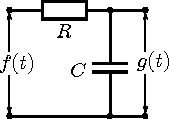
\includegraphics[scale=0.8]{Chapter_6/v6-RC.pdf}
\caption{\footnotesize Интегрирующая $RC$-цепочка}
\figmark{RC}
\end{wrapfigure}

\begin{exmpl}\label{exmpl:RC}
Найдём частотную характеристику $RC$-цепочки (рис.~\figref{RC}).
Повторяя рассуждения из Примера~\ref{exmpl:RLC} при $L=0$, получим
\[
\lambda(\omega) = \frac{1}{1+i\omega \tau_C},
\]
где $\tau_C=RC$ --- постоянная времени $RC$-цепочки.

При $\omega \gg 1/\tau_C$ имеем $\lambda \approx \frac{1}{i\omega\tau_C} \to 0$,
то есть $RC$-цепочка является простейшим \important{фильтром высоких частот}.

В этом пределе можно выразить результат действия цепочки в явном виде.
При $\omega\tau_C\gg1$ напряжение на конденсаторе $q/C$ мал\'{о} по сравнению
с напряжением $\dot{q}R$ на резисторе, поэтому
\[
\dot{q} R \approx f(t) \qquad \to \qquad g(t) = \frac{q}{C} = \frac{1}{\tau_C}\int\limits_0^t f(t')\,dt'.
\]
Таким образом, фильтрация высокочастотных гармоник сводится к интегрированию
входного сигнала (подумайте, почему интеграл от быстропеременной функции
по достаточно большому интервалу оказывается мал).
\end{exmpl}

\introsection{Спектральное разложение}

Итак, при изучении линейных систем (фильтров) возникает необходимость
представления произвольного сигнала $f(t)$ в виде
\begin{equation}
    \eqmark{Fourier series}
    f(t)=\sum\limits_n c_n e^{i\omega_n t}.
\end{equation}
Представление \eqref{Fourier series} называется разложением сигнала~$f(t)$ в
\term{ряд Фурье}, а отдельные слагаемые ряда (составляющие
гармонические колебания) $c_n e^{i\omega_n t}$ называют \term{гармониками}.
Совокупность коэффициентов~$\{c_n\}$ называется \term{спектром} функции~$f(t)$.
Коэффициент~$c_n$ представим в виде $c_n=a_ne^{i\varphi_n}$, где
модуль $a_n=|c_n|$ определяет \important{амплитуду} гармоники частоты~$\omega_n$,
а аргумент $\varphi_n=\arg c_n$~--- \important{начальную фазу}.

В курсах математического анализа доказывается, что
разложение~\eqref{Fourier series} может быть осуществлено в общем случае (при
некоторых физически несущественных
ограничениях на~$f(t)$), причем \important{единственным} образом.
То есть, существует единственный набор необходимых частот~$\omega_n$ и
единственный набор отвечающих этим частотам амплитуд~$a_n$ и фаз~$\varphi_n$,
обеспечивающих представление функции~$f(t)$ в виде суперпозиции гармонических
функций. Соответствующие формулы для этих коэффициентов мы получим ниже.

Отметим важное свойство гармонических функций.
Колебание $e^{i\omega_0 t}$ частоты~$\omega_0$ не может быть
представлено суперпозицией гармонических колебаний $\sum c_n e^{i\omega_n t}$
других частот $\omega_n\ne\omega_0$, какие бы коэффициенты~$c_n$, т.\,е.
амплитуды и фазы слагаемых гармоник, мы ни подбирали. В~математике это
свойство называют \term{ортогональностью}: функция $e^{i\omega_0 t}$
не имеет <<проекции>> на любую другую функцию $e^{i\omega_nt}$ при
$\omega_0\ne\omega_n$ (подобно тому как вектор, параллельный оси~$z$,
невозможно представить в виде суммы векторов, параллельных осям~$x$ и~$y$).

Для \important{действительных} функций $f(t)$, которые как правило и представляют интерес,
наряду с разложением \eqref{Fourier series} часто используется разложение
в ряд Фурье вида%
\footnote{Также можно использовать эквивалентное разложение
\[f(t)=\sum\limits_{n=0}^{\infty} A_n \cos(\omega_n t) + B_n \sin(\omega_n t),\]
где $a_n=\sqrt{A_n^2+B_n^2}$, $\tg \varphi_n = \frac{B_n}{A_n}$.}
\begin{equation}
    \eqmark{Fourier-real-valued function}
    f(t)=\sum\limits_{n=0}^{\infty} a_n \cos(\omega_n t+\varphi_n ),
\end{equation}
где $a_n$, $\varphi_n$~--- действительные константы. Найдём связь между
коэффициентами разложений \eqref{Fourier series} и \eqref{Fourier-real-valued function}.
Пользуясь формулой Эйлера
\begin{equation}
    \eqmark{euler}
    \cos\alpha=\frac{e^{i\alpha}+e^{-i\alpha}}{2},
\end{equation}
представим каждое слагаемое \eqref{Fourier-real-valued function} в виде
\begin{equation*}
    a_n\cos(\omega_nt+\varphi_n)=\frac{a_n}{2}e^{i\varphi_n}\,e^{i\omega_n
t}+\frac{a_n}{2}e^{-i\varphi_n}\,e^{-i\omega_n t},
\end{equation*}
откуда ясно, что разложения \eqref{Fourier series} и
\eqref{Fourier-real-valued function} будут тождественны, если суммирование в
\eqref{Fourier series} проводить как по положительным частотам~$\omega_n$
(имеющим понятный физический смысл), так и по отрицательным (формально введённым)
частотам $\omega_{-n}=-\omega_n$, причём соответствующие коэффициенты имеют вид
\begin{equation}
    \eqmark{Fourier-coefficient}
    c_n =\frac{1}{2}a_n e^{i\varphi_n},
    \qquad c_{-n}=\frac{1}{2}a_n e^{-i\varphi_n}
\end{equation}
(коэффициенты $c_{-n}$ соответствуют отрицательным частотам~$-\omega_n)$,
т.\,е каждому слагаемому $a_n\cos(\omega_nt+\varphi_n)$ ряда \eqref{Fourier series}
соответствуют два слагаемых $c_ne^{i\omega_n t}$ и
$c_{-n}e^{-i\omega_n t}$ ряда \eqref{Fourier-real-valued function}.
% Нетрудно получить формулы обратного перехода от $\{c_n\}$ к
% $\{a_n,\varphi_n\}$:
% \begin{equation}
%      \eqmark{Fourier-coefficient-reverse}
%     a_n = 2|c_n|\qquad \varphi_n = \arg c_n.
% \end{equation}


Мы видим, что при разложении \important{действительных} функций~$f(t)$ в ряд Фурье
коэффициенты разложения~$c_{-n}$ на отрицательных
частотах связаны с коэффициентами~$c_n$ простым соотношением
\[
c_{-n}=c_{n}^*,
\]
где звёздочка обозначает \important{комплексное сопряжение}.
Таким образом, гармоники с отрицательными частотами не несут какой-либо
дополнительной информации о действительном сигнале~$f(t)$.

Спектр функции~$f(t)$ принято изображать в виде графика
(рис.~\figref{spectrum}): длина стрелочки на каждой частоте~$\omega_n$
определяется модулем коэффициента~$c_n$ (т.~е. амплитудой соответствующего
гармонического колебания). Следует указать также начальные фазы~$\varphi_n$
спектральных компонент.

\begin{figure}[ht]
%     \psfragfig[width=0.7\textwidth]{Images/Chapter_6/7}{%
%     \psfrag{a}[ct]{$\omega_1$}
%     \psfrag{b}[ct]{$\omega_2$}
%     \psfrag{c}[ct]{$\omega_3$}
%     \psfrag{d}[ct]{$\omega_4$}
%     \psfrag{e}[ct]{$-\omega_{1}$}
%     \psfrag{f}[ct]{$-\omega_{2}$}
%     \psfrag{g}[ct]{$-\omega_{3}$}
%     \psfrag{h}[ct]{$-\omega_{4}$}
%     \psfrag{o}[ct]{0}
%     \psfrag{1}[cb]{$\varphi_1$}
%     \psfrag{2}[cb]{$\varphi_2$}
%     \psfrag{3}[cb]{$\varphi_3$}
%     \psfrag{4}[cb]{$\varphi_4$}
%     \psfrag{x}{$\omega$}
%     \psfrag{y}{$\{c_n\}$}
%     \psfrag{z}{$\{a_n\}$}
%     \psfrag{A}{а)}
%     \psfrag{B}{б)}}
    \centering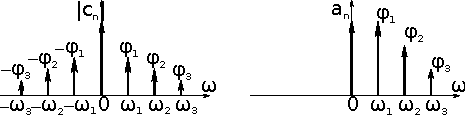
\includegraphics{Chapter_6/v6-cmplx-vs-real.pdf}
    \caption{Спектр в комплексном (слева) и действительном (справа) представлениях}
    \figmark{spectrum}
\end{figure}

Пример разложения \eqref{Fourier-real-valued function} (в ряд
косинусов) представлен на графике рис. \figref{spectrum} (справа): здесь нет
отрицательных частот, а длины стрелочек на положительных частотах в соответствии с
\eqref{Fourier-coefficient} удваиваются. При этом постоянные составляющие
(на частоте $\omega=0$) в разложениях \eqref{Fourier series} и
\eqref{Fourier-real-valued function} одинаковы: $a_0=c_0$.

\introsubsection{Спектр периодического процесса}\label{sec:spectrum-periodic}
Получим коэффициенты разложения в ряд Фурье для периодического колебательного
процесса общего вида $f(t)=f(t+T)$, где $T$~--- период процесса.
Покажем, что в этом случае функция~$f(t)$ может быть представлена
бесконечной суммой гармонических колебаний с кратными частотами~$\omega_n=n\omega_0$,
где $\omega_0=2\pi/T$, $n$~--- целое число:
\begin{equation}
    \eqmark{Fourier-periodic osc}
    f(t)=\sum_{n=-\infty}^{\infty} c_n e^{in\omega_0 t}.
\end{equation}
Нетрудно видеть, что все слагаемые в \eqref{Fourier-periodic osc}~---
периодические функция с периодом, кратным $T$, и они полностью исчерпывают
набор гармонических функций, удовлетворяющих условию $f(t)=f(t+T)$.
Таким образом, периодическая функция имеет \term{дискретный}
спектр с кратными частотами.

Спектр --- то есть набор коэффициентов~$\{c_n\}$ ---
можно найти следующим образом: домножим обе части равенства
\eqref{Fourier-periodic osc} на $e^{-im\omega_0 t}$ и
проинтегрируем по времени~$t$ за период (например от~$0$ до~$T$). Получим
\begin{equation*}
    \int\limits_{0}^{T} f(t)e^{-im\omega_0t}\,dt=\sum_n c_n\int\limits_{0}^{T}
e^{i(n-m)\omega_0 t}\,dt.
\end{equation*}
Вычислим интеграл в правой части:
\begin{equation*}
    \int\limits_{0}^{T}e^{i(n-m)\omega_0 t}dt =
%     = \left.\frac{e^{i(n-m)\omega_0 t}}{i(n-m)\omega_0} \right|_0^{T}
    \begin{cases}
        0 & \text{при~}n\ne m,\\
        T & \text{при~}n = m.
    \end{cases}
\end{equation*}
% (время $T$ есть целое число периодов колебания функций
% $\cos(n-m)\omega_0t$ и $\sin(n-m)\omega_0t$, поэтому интегралы от них
% на отрезке $[0,\,T]$ зануляются).
Таким образом, находим
\begin{equation}
    \eqmark{fourier-coeff}
    c_n=\frac{1}{T}\int\limits_{0}^{T} f(t)e^{-in\omega_0 t}\,dt.
\end{equation}
Это и есть искомое правило нахождения коэффициентов разложения периодической
функции в гармонический ряд Фурье.

\begin{wrapfigure}[10]{o}{0.5\textwidth}
%     \psfragfig[width=0.5\textwidth]{Images/Chapter_6/12}{%
%     \psfrag{x}{$t$}
%     \psfrag{1}[rb]{1}
%     \psfrag{f}{$f(t)$}
%     \psfrag{a}[cb]{$\tau$}
%     \psfrag{b}[cb]{$T$}}
\centering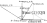
\includegraphics[width=0.5\textwidth]{Chapter_6/12}
    \caption{\footnotesizeПериодическая последовательность импульсов}
    \figmark{meander}
\end{wrapfigure}

\begin{exmpl}\label{exmpl:square-zug}
Найдём спектр периодической последовательности прямоугольных
импульсов длительности~$\tau$ с периодом следования импульсов $T>\tau$
(рис.~\figref{meander}, начало отсчёта выбрано так, что~$f(t)$ --- чётная
функция).

Используя \eqref{fourier-coeff} на интервале интегрирования
$-T/2\le t \le T/2$, с учётом того, что функция~$f(t)$ отлична от нуля и
равна единице лишь в области $|t|<\tau/2$, находим
\begin{equation}
    \eqmark{impulses-spectrum}
    c_n =\frac{1}{T}\int\limits_{-\tau/2}^{\tau/2} e^{-in\omega_0 t}\,dt
    =\frac{\tau}{T}\cdot \frac{\sin \left(n\omega_0\tau/2\right)}{n\omega_0\tau/2} =
     \frac{\sin \left(\pi n \tau/T\right)}{\pi n}.
\end{equation}

\begin{figure}[h!]
%     \psfragfig[width=\textwidth]{Images/Chapter_6/13}{%
%     \psfrag{x}{$\omega$}
%     \psfrag{y}{$c_n$}
%     \psfrag{0}[tr]{0}
%     \psfrag{1}[ct]{$\vphantom{2}\omega_0$}
%     \psfrag{2}[ct]{$2\omega_0$}
%     \psfrag{c}{$C(\omega)$}
%     \psfrag{d}[ct]{$2\Delta\omega$}}
\centering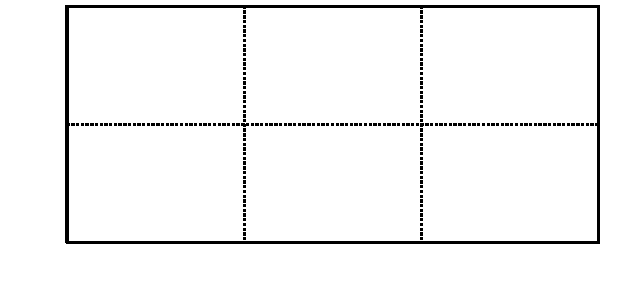
\includegraphics[width=0.9\textwidth]{Chapter_6/13.pdf}
    \caption{Спектр периодической последовательности импульсов
        (рисунок приведён для случая $\tau=\frac13 T$)}
    \figmark{spectrum-meander}
\end{figure}

Спектр $\{c_n\}$ показан на рис.~\figref{spectrum-meander}.
Пунктирной кривой изображена огибающая функция
\begin{equation*}
    C(\omega) =\frac{\tau}{T}\cdot \frac{\sin\omega\tau/2}{\omega\tau/2}.
\end{equation*}
При $\omega=n\omega_0$ эта функция принимает значение $C(n\omega_0)=c_n$.
Полуширина $\Delta \omega$ главного максимума этой функции определяется
условием $\sin\omega\tau/2=0$:
\begin{equation*}
    \Delta\omega \cdot \frac{\tau}{2}=\pi\qquad \text{или} \qquad \Delta \omega
\cdot \tau =2\pi.
\end{equation*}
Как видно из рисунка, спектральные гармоники,
имеющие заметную амплитуду, сосредоточены в интервале частот
$|\omega|\lesssim\Delta\omega=2\pi/\tau$.
\end{exmpl}


\introsubsection{Спектр непериодического процесса}

Рассмотрим задачу разложения в спектр произвольного непериодического
сигнала $f(t)$.

Ответ можно получить, воспользовавшись результатом
\eqref{fourier-coeff} для разложения периодической функции
и устремляя период к бесконечности $T\to \infty$.

\begin{wrapfigure}[9]{o}{0.5\textwidth}
    \centering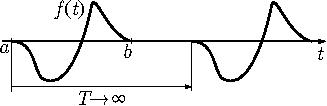
\includegraphics[width=\linewidth]{Chapter_6/v6-finf.pdf}
    \caption{Непериодический процесс как предел периодического}
    \figmark{finf}
\end{wrapfigure}

Пусть функция $f(t)$ отлична от нуля на некотором конечном интервале
$t\in[a,\,b]$, а вне его обращается в ноль. Рассмотрим периодическую функцию
с достаточно большим периодом повторения $T>b-a$, составленную из <<кусков>>
функции $f(t)$. Посмотрим, что происходит со спектральным разложением
такой функции по мере увеличения $T$.

Видно, что частоты $\omega = n \frac{2\pi}{T}$ гармоник, по которым идёт
разложение, будут в пределе $T\to \infty$ располагаться всё плотнее друг к другу.
Интервал между соседними частотами равен $\Delta \omega = \frac{2\pi}{T}$.
Таким образом, имеем $\Delta \omega\to 0$ и, следовательно,
спектр должен стать \term{непрерывным}.

Тогда спектральное разложение превратится из суммы в интеграл:
\[
 f(t) = \frac{1}{\Delta \omega}\sum c_n e^{i\omega_n t} \Delta \omega \to
 \frac{T}{2\pi} \int\limits_{-\infty}^{\infty} c_n e^{i\omega_n t} d\omega,
\]
Обозначая $C(\omega)=c_n T$, запишем искомое разложение как
\begin{equation}
\eqmark{Fourier integral}
f(t) = \frac{1}{2\pi} \int\limits_{-\infty}^{\infty} C(\omega) e^{i\omega t} d\omega,
\end{equation}
где $C(\omega)$ найдём из \eqref{fourier-coeff}:
\begin{equation}
\eqmark{Fourier integral-coef}
 C(\omega) =
%  \frac{c_n}{\Delta \omega} =
%  \frac{1}{\Delta \omega T}\int\limits_{-\infty}^{\infty}
%  f(t) e^{-i\omega t} dt \to
\int\limits_{-\infty}^{\infty} f(t) e^{-i\omega t} dt.
\end{equation}

Множитель $C(\omega)=a(\omega)e^{i\varphi(\omega)}$ показывает, с каким
<<весом>> (т.~е. с какой амплитудой $a(\omega)$ и с какой начальной фазой
$\varphi(\omega)$) необходимо складывать гармонические
колебания разных частот, чтобы при суммировании (интегрировании) образовать
заданный сигнал $f(t)$. Функция $C(\omega)$ называется \term{спектром}
или \term{преобразованием Фурье} сигнала~$f(t)$.
Видно, что в общем случае необходим непрерывный набор (\important{континуум}) гармоник.

Соотношение \eqref{Fourier integral-coef} также называют
\term{прямым преобразованием Фурье}, а формулу \eqref{Fourier integral}~---
\term{обратным преобразованием Фурье}.
Связь функцией и её спектром символически можно записать как
\[
C(\omega) = \hat{\mathcal{F}}[f(t)],\qquad f(t) = \hat{\mathcal{F}}^{-1}[C(\omega)],
\]
где $\hat{\mathcal{F}}$ и~$\hat{\mathcal{F}}^{-1}$~--- условное обозначение
для прямого и обратного преобразования Фурье (заметим, что
эти преобразования \important{линейны}).

\begin{exmpl}\label{exmpl:square}
Найдём спектр прямоугольного импульса длительности $\tau$
единичной амплитуды (рис.~\figref{spectrum-one meander}а). Используя
\eqref{Fourier integral-coef}, получаем
\begin{equation}
    \eqmark{spectrum-impulse}
    C(\omega)=\int\limits_{-\tau/2}^{\tau/2} e^{-i\omega
t}\,dt=\frac{1}{-i\omega}\int\limits_{-\tau/2}^{\tau/2} e^{-i\omega t}\,
d(-i\omega t)=\tau\frac{\sin\omega\tau/2}{\omega\tau/2}.
\end{equation}
Функция $C(\omega)$ показана на рис.~\figref{spectrum-one meander}б.
\begin{figure}[h!]
   \centering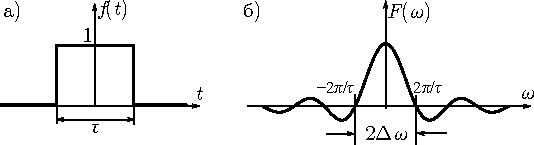
\includegraphics{Chapter_6/v6-single.pdf}
    \caption{Одиночный импульс (а) и его спектр (б)}
    \figmark{spectrum-one meander}
\end{figure}

Полезно сравнить спектр отдельного импульса со спектром периодической
последовательности одинаковых импульсов (рис.~\figref{spectrum-meander}).
Вместо \important{дискретного} спектра $\{c_n\}$ мы получили
\important{непрерывный} спектр~$C(\omega)$, причём
спектр импульса $C(\omega)$ (с множителем $1/T$) представляет собой
<<огибающую>> частокола спектральных компонент $c_n$
периодической последовательности импульсов.

Заметим также, что, как видно из графика, основной вклад дают гармоники, частоты
которых заполняют интервал $|\Delta\omega|<2\pi/\tau$. Это~--- полуширина
главного максимума функции $\frac{\sin\omega\tau/2}{\omega\tau/2}$. Диапазон
частот $\Delta\omega$ можно назвать характерной \important{шириной спектра}
$C(\omega)$.
\end{exmpl}


\introsubsection{Соотношение неопределённостей}
\label{sec:indeterminacy}

При рассмотрении Примеров~\ref{exmpl:square-zug} и~\ref{exmpl:square},
мы получили замечательное соотношение, связывающее между собой
длительность~$\Delta t$ сигнала с шириной его спектра~$\Delta \omega$:
\begin{equation}
    \eqmark{indeterminacy relation}
    \Delta t \cdot \Delta\omega \sim 2\pi.
\end{equation}

Оказывается, это соотношение имеет универсальный характер.
Оно остаётся справедливым по порядку величины для произвольного сигнала $f(t)$.
% (соответствующую строгую теорему можно найти в курсах математического анализа).
Чем больше длительность сигнала~$\Delta t$ (либо больше интервал времени,
в течение которого происходит его заметное изменение), тем \'{у}же спектр
сигнала~$\Delta\omega$, и, наоборот, чем короче сигнал (или быстрее происходит
изменение сигнала), тем шире его спектр, т.\,е. требуется более широкий интервал
частот гармонических колебаний, образующих в сумме данный сигнал.
В этом состоит смысл формулы \eqref{indeterminacy relation},
которая называется \term{соотношением неопределённостей}.

В общем случае, если у сигнала есть какое-то характерное время~$\Delta t$,
в его спектре обязательно возникнет некоторый характерный масштаб
$\Delta \omega \sim 2\pi /\Delta t$. Например, рассмотрим ограниченную
последовательность периодических импульсов с полной длительностью~$t_0$,
периодом~$T\ll t_0$ и длительностью каждого импульса~$\tau\ll T$.
Сигнал и его спектр представлены на рис.~\figref{indeterm}
(он может быть без труда рассчитан из формулы \eqref{Fourier integral-coef}
с использованием результатов разобранных выше Примеров~\ref{exmpl:RLC}
и~\ref{exmpl:square-zug}). На спектре видно три характерных масштаба частоты:
наибольший масштаб~$\Delta \omega_{\tau} = 2\pi/\tau$ задаёт ширину всего спектра,
масштаб~$\Delta \omega_T = 2\pi / T$ есть расстояние между соседними
спектральными пиками, и наконец наименьший машстаб $\Delta \omega_0 = 2\pi /t_0$,
соответствующий наибольшему характерному времени~$t_0$,
определяет ширину каждого пика.

\begin{figure}[h!]
\centering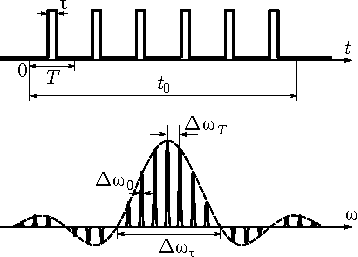
\includegraphics[scale=1.0]{Chapter_6/v6-indeterm.pdf}
\caption{Связь ширины спектра с характерными временными масштабами}
\figmark{indeterm}
\end{figure}

\introsubsection{Спектральный метод в задаче линейной фильтрации}

Сформулируем ещё раз алгоритм решения задачи линейной фильтрации
спектральным методом (методом Фурье) с учётом полученных соотношений.

Для нахождения отклика линейной системы $g(t)$ на воздействие $f(t)$
нужно:
\begin{enumerate}
    \item представить входной сигнал $f(t)$ в виде ряда
    \eqref{Fourier series} или интеграла Фурье \eqref{Fourier integral},
где спектр $\hat{\mathcal{F}}[f]$ (функция $C(\omega)$ или набор $\{c_n\}$)
находится с помощью соотношений \eqref{fourier-coeff}
или~\eqref{Fourier integral-coef};

    \item найти частотную характеристику фильтра
$\lambda(\omega)$, т.\,е. функцию отклика фильтра на гармоническое внешнее воздействие
единичной амплитуды:
\begin{equation*}
    e^{i\omega t}\to\fbox{$\hat\Lambda$}\to \lambda(\omega)e^{i\omega t};
\end{equation*}

    \item просуммировать отклики на каждое гармоническое
    слагаемое входного сигнала, что даёт спектр выходного сигнала:
    \begin{equation*}
    \sum c_n e^{i\omega_n t} \to\fbox{$\hat\Lambda$}\to \sum \lambda(\omega_n)c_n e^{i\omega_n t},
    \end{equation*}
    или
    \begin{equation*}
    \int C(\omega) e^{i\omega t} \to\fbox{$\hat\Lambda$}\to
    \int \lambda(\omega)\cdot C(\omega)e^{i\omega t};
    \end{equation*}
    \item восстановить выходной сигнал $g(t)$ по его спектру
    (обратное преобразование Фурье).
\end{enumerate}
Всю схему можно записать кратко одной формулой:
    \begin{equation}
        \eqmark{linear-filter-fourier}
    g(t) = \hat{\mathcal{F}}^{-1}\!
    \left[\lambda(\omega)\cdot \hat{\mathcal{F}}[f(t)]\right].
    \end{equation}


\begin{wrapfigure}[14]{o}{0.25\textwidth}
     \centering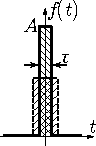
\includegraphics{Chapter_6/v6-delta.pdf}
     \caption{\footnotesize Предельный переход к дельта-импульсу}
\end{wrapfigure}

\begin{exmpl}\label{exmpl:delta}
Устремим длительность импульса из предыдущего примера к нулю $\tau\to 0$,
при этом его амплитуду $A$ будем наращивать так, чтобы площадь
под его графиком оставалась постоянной (единичной): $\int f(t) = A \tau = 1$.
Такой импульс физике обозначают как $\delta(t)$ и называют \important{дельта-импульсом}
(или \important{дельта-функцией}).

Поскольку $\sin x/x\to 1$ при $x\to 0$,
предельный переход \eqref{spectrum-impulse} даёт простой результат:
\begin{equation}
    \eqmark{spectrum-delta}
    C(\omega)\to A\tau =1.
\end{equation}
То есть спектр бесконечно узкого импульса единичной площади (дельта-функции)
есть единичная константа. Заметим, что и здесь выполняется соотношение
неопределённостей: бесконечно узкий импульс даёт бесконечно широкий спектр.

Этот результат позволяет придать новый смысл частотной характеристике
(функции отклика) $\lambda(\omega)$ некоторого фильтра.
Если спектр входного сигнала $f(t)$ есть единичная константа,
то как следует из соотношения \eqref{linear-filter-fourier},
откликом системы будет функция $g(t)$, спектр которой совпадает
с $\lambda(\omega)$. Таким образом, \important{обратное преобразование Фурье
от функции отклика системы есть её реакция на единичный дельта-имульс}.
\end{exmpl}


\introsubsection{Физический смысл спектрального разложения}
\label{sec:spectrum-meaning}

Разложение функции $f(t)$ в ряд или интеграл Фурье может показаться
абстрактной математической операцией --- некоторым трюком, не имеющим
под собой физического содержания. Попробуем ответить на вопрос,
можно ли \important{измерить} амплитуды спектральных компонент $f(t)$,
тем самым приписав им прозрачный физический смысл.

Рассмотрим колебательный $RLC$-контур и подадим на его вход некоторый сигнал $f(t)$.
Для простоты ограничимся периодической функцией.

Пусть собственная частота контура равна $\Omega$, а добротность его
достаточно велика: $Q=\Omega/2\gamma \gg 1$ ($\gamma$ --- коэффициент затухания).

Пусть известно спектральное разложение $f(t)=\sum c_n e^{i\omega_n t}$.
После <<фильтрации>> через контур на выходе получим сигнал со
спектральными компонентами $g(t)=\sum g_n e^{i\omega_n t}$,
где $g_n = \lambda(\omega_n) c_n$ для каждого $n$,
$\lambda(\omega)$ --- частотная характеристика $RLC$-контура, найденная
выше (см. Пример~\ref{exmpl:RLC}). Нетрудно видеть, что такое преобразование резко
(примерно в $Q$ раз) усиливает частоты входного сигнала, близкие к
$\Omega$ (т.\,е. к \important{резонансу}), и ослабляет далёкие.
В~пределе идеального контура ($Q\to \infty$), в спектре сигнала на выходе
останется единственная~--- резонансная~--- частота.
Сигнал $g(t)$ будет гармоническим колебанием с частотой $\Omega$:
$g(t) \propto c(\Omega) e^{i\Omega t}$,
причём его амплитуда будет пропорциональна амплитуде гармоники с этой
частотой в разложении исходной функции $f(t)$ (а если в этом разложении не было
гармоники $\omega_n=\Omega$, результирующая амплитуда будет нулевой).

Мы видим, что высокодобротный колебательный контур <<отфильтровывает>> из подаваемого
на него сигнала те спектральные компоненты, частоты которых близки к
его собственной $\Omega$. По амплитуде отклика можно измерить и амплитуду
гармоники в исходном сигнале. Меняя собственную частоту контура $\Omega$
(например, изменяя ёмкость конденсатора), можно в принципе просканировать весь
диапазон частот, измерив таким образом амплитуды всех спектральных
компонент~$c_n$ в разложении $f(t)=\sum c_n e^{i\omega_n t}$. Итак,
спектр сигнала может быть измерен непосредственно и описанная схема измерения
позволяет придать спектральному разложению наглядный физический смысл.

\begin{exmpl}\label{exmpl:zug-RLC}
Рассмотрим колебательный $RLC$-контур с собственной
частотой~$\Omega$ и добротностью $Q\gg 1$, в котором мы попытаемся раскачать колебания,
подавая на вход периодическую последовательность коротких импульсов
с периодом $T$ и длительностью $\tau$. Можно ли раскачать колебания в контуре
до сколь-нибудь значимых амплитуд, если частота повторения импульсов
$\omega_0=2\pi/T$ много меньше резонасной частоты контура $\Omega$,
$\omega_0\ll \Omega$?

\begin{figure}[h!]
 \centering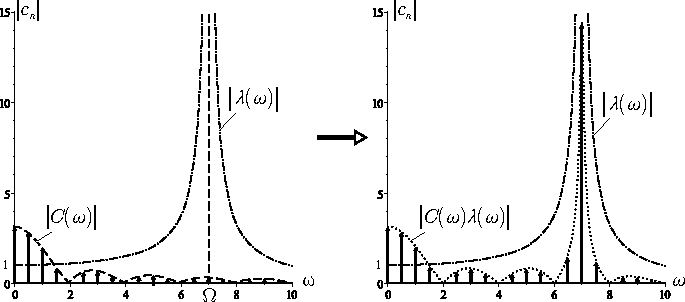
\includegraphics[width=\textwidth]{Chapter_6/v6-impulse-filter.pdf}
 \caption{\footnotesize Изменение спектра периодической последовательности импульсов (слева)
 в результате фильтрации колебательным контуром (справа) при резонансе с одной
 из высокочастотных гармоник. Расчёт проведён
 для $Q=50$, $\omega_0=\Omega/7$, $\tau=T/4$}
 \figmark{impulse-filter}
\end{figure}

Для нахождения амплитуды результирующих колебаний нужно перемножить
спектр периодической последовательности $\{c_n\}$
(см. Пример~\ref{exmpl:square-zug}, \eqref{impulses-spectrum})
и частотную характеристику колебательного контура $\lambda(\omega)$
(см. Пример~\ref{exmpl:RLC}, \eqref{RLC-lambda}).
Возможный результат такого преобразования представлен на рис.~\figref{impulse-filter}.
Видно, что благодаря существованию в спектре входного сигнала высокочастотных
гармоник $\omega_n = n \omega_0$, при выполнении условия
$\Omega = n \omega_0$, где $n$ --- целое, и при достаточно высокой добротности,
такая раскачка колебаний возможна.

Из \eqref{impulses-spectrum} видно, что амплитуды гармоник $|c_n|$ убывают
с ростом $n$ как $1/n$. С другой стороны, из \eqref{RLC-lambda} можно получить,
что в резонансе сигнал усиливается в $Q$ раз.
Таким образом, раскачать колебания в высокодобротном $RLC$-контуре можно
с помощью периодических импульсов, частота повторения $\omega_0=2\pi/T$
которых может быть существенно меньше резонансной,
вплоть до $\omega_0 \sim \Omega / Q \ll \Omega $.
\end{exmpl}

\introsubsection[Свойства преобразования Фурье]{%
    Свойства преобразования Фурье}
% \protect\footnote{При первом чтении данный раздел можно пропустить.}}

Рассмотрим некоторые свойства спектрального разложения (преобразования Фурье),
которые могут быть полезны при расчёте спектров.

\begin{wrapfigure}{o}{0.3\textwidth}
 \centering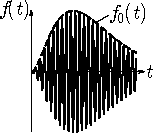
\includegraphics{Chapter_6/v6-modul.pdf}
 \caption{}
 \figmark{modul}
\end{wrapfigure}

\paragraph{Спектр огибающей, заполненной высокочастотным сигналом.}
Пусть $C_0(\omega)$ --- спектр некоторой функции $f_0(t)$.
Найдём спектр $C(\omega)$ функции
\[
f(t)=f_0(t)\cos(\omega_0 t).
\]
Здесь $f_0(t)$ имеет смысл <<огибающей>>, заполненной колебаниями
с частотой~$\omega_0$ (см. рис.~\figref{modul}).

Используя формулу Эйлера \eqref{euler}, запишем
\begin{equation*}
    f(t)=\frac{1}{2}f_0(t)e^{i\omega_0t}+\frac{1}{2}f_0(t)e^{-i\omega_0t}.
\end{equation*}
Пользуясь \eqref{Fourier integral-coef}, найдём спектр
функции $f_0(t)e^{i\omega_0 t}$:
\begin{equation}
    \eqmark{task-spectrum-shift}
%     \int\limits_{-\infty}^\infty f_0(t)e^{i\omega_0 t}\cdot e^{-i\omega
% t}\,dt=
    \hat{\mathcal{F}}[f_0(t)e^{i\omega_0 t}]=
\int\limits_{-\infty}^\infty
f_0(t)e^{-i(\omega-\omega_0)t}\,dt=C_0(\omega-\omega_0),
\end{equation}
т.~е. при умножении на $e^{i\omega_0 t}$ исходный спектр
\important{сдвигается} по оси частот на величину $\omega_0$
(рис.~\figref{task-shift-spectrum}).

\begin{figure}[h!]
\centering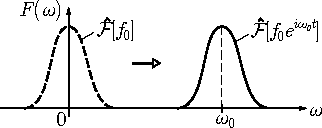
\includegraphics{Chapter_6/v6-shift.pdf}
\caption{Смещение спектра при домножении сигнала на $e^{i\omega_0 t}$}
\figmark{task-shift-spectrum}
\end{figure}

%\begin{equation}
%   \eqmark{task-freq-shift}
%   C(\omega)=e^{-i\omega\tau}\int_{-\infty}^\infty f_0(t')e^{-i\omega
% t'}\,dt'=C_0(\omega)\cdot e^{-i\omega\tau},
%\end{equation}
%или символически $f_0(t-\tau) \leftrightarrow C_0(\omega)e^{-i\omega\tau}$,
% т.е. смещение сигнала во времени на $\tau$ (запаздывание) приводит к умножению
% его спектра на $e^{-i\omega\tau}$ (теорема смещения).
%

Отсюда находим искомый спектр:
\begin{equation}
    \eqmark{task-2shift-spectrum-cos}
    C(\omega)=\frac{1}{2}C_0(\omega-\omega_0)+\frac{1}{2}C_0(\omega+\omega_0).
\end{equation}
Если частота $\omega_0$ существенно превосходит характерную ширину $\Delta \omega$
спектра огибающей, $\omega_0 \gg \Delta \omega$, то слагаемые
\eqref{task-2shift-spectrum-cos} не накладываются друг на друга.
Тогда искомый спектр $C(\omega)$ получается из $C_0(\omega)$
простым смещением по оси частот влево и вправо на <<несущую>>
частоту $\omega_0$ (с домножением на 1/2, см. рис.~\figref{task-2shift-spectrum-cos}).

\begin{figure}[h!]
%     \psfragfig[width=0.8\textwidth]{Images/Chapter_6/15b}{%
%     \psfrag{x}{$\omega$}
%     \psfrag{y}{$C_0(\omega)$}
%     \psfrag{z}{$C(\omega)$}
%     \psfrag{a}[ct]{$-\omega_0$}
%     \psfrag{b}[ct]{$\omega_0$}}
\centering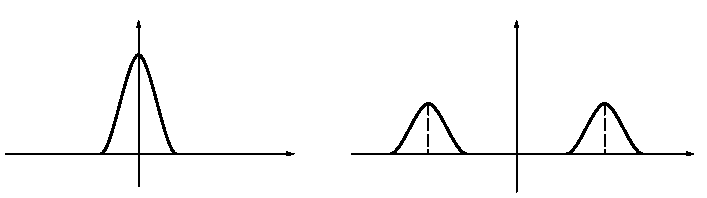
\includegraphics[width=0.8\textwidth]{Chapter_6/15b.pdf}
    \caption{Преобразование спектра при домножении на $\cos \omega_0 t$}
    \figmark{task-2shift-spectrum-cos}
\end{figure}

\begin{wrapfigure}{o}{0.5\textwidth}
%     \psfragfig[width=0.5\textwidth]{Images/Chapter_6/16}{%
%     \psfrag{t}{$t$}
%     \psfrag{f}{$f_0(t)$}
%     \psfrag{F}{$f(t)$}
%     \psfrag{a}[ct]{$\llap{$-$}\frac{\tau}{2}$}
%     \psfrag{b}[ct]{$\frac{\tau}{2}$}
%     \psfrag{A}{а)}
%     \psfrag{B}{б)}}
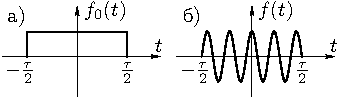
\includegraphics[width=0.5\textwidth]{Chapter_6/16}
    \caption{\footnotesize Прямоугольный импульс (а), ограничивающий синусоиду (б)}
    \figmark{one-zug}
\end{wrapfigure}

\begin{exmpl}\label{exmpl:one-zug}
Найдём спектр обрывка синусоиды с частотой $\omega_0$
длительностью $\tau$ (такой сигнал называют \term{цугом}).
Сигнал может быть представлен как
\[f(t)=f_0(t)\cos(\omega_0 t),\] где $f_0(t)$ --- единичный прямоугольный
импульс длительностью $\tau$ (см. рис.~\figref{one-zug}).

Пользуясь полученными ранее формулами для спектра прямоугольного импульса
\eqref{spectrum-impulse} и для смещения спектра \eqref{task-2shift-spectrum-cos},
получим
\begin{equation*}
C(\omega)=\frac{\tau}{2}\left[\frac{\sin(\omega-\omega_0)\tau/2}{
(\omega-\omega_0)\tau/2}+
\frac{\sin(\omega+\omega_0)\tau/2}{(\omega+\omega_0)\tau/2}
\right].
\end{equation*}
Спектры $C_0(\omega)$ и $C(\omega)$ представлены на
рис.~\figref{task-meander-train-spectrum}.

\begin{figure}[h!]
%     \psfragfig[width=0.8\textwidth]{Images/Chapter_6/17}{%
%     \psfrag{p}[br]{$\tau$}
%     \psfrag{q}{$\tau/2$}
%     \psfrag{w}{$\omega$}
%     \psfrag{f}{$C_0(\omega)$}
%     \psfrag{F}{$C(\omega)$}
%     \psfrag{a}[ct]{$\llap{$-$}\omega_0$}
%     \psfrag{b}[ct]{$\omega_0$}
%     \psfrag{A}{а)}
%     \psfrag{B}{б)}}
\centering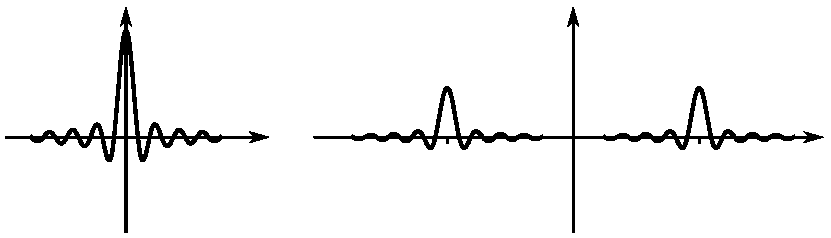
\includegraphics[width=0.8\textwidth]{Chapter_6/17}
    \caption{Спектры а) прямоугольного импульса, б) импульса,
        заполненного синусоидой (цуга)}
    \figmark{task-meander-train-spectrum}
\end{figure}
\end{exmpl}


\begin{exmpl}\label{exmpl:exp}
Найдём спектр затухающих колебаний
\[
f(t) = e^{-\gamma t} \sin \omega_0 t\qquad (\text{при~}t\ge 0).
\]
По формуле \eqref{Fourier integral-coef} находим спектр затухающей
экспоненты (начинающейся с $t=0$):
\[
\hat{\mathcal{F}}[e^{-\gamma t}] =
\int\limits_0^{\infty} e^{-\gamma t - i\omega} dt =
\frac{1}{\gamma + i\omega}
\]
(ср. с Примером~\ref{exmpl:RC}).
Пользуясь формулой Эйлера для синуса
\[
\sin \alpha = \frac{e^{i\alpha} - e^{-i\alpha}}{2i},
\]
получим искомый спектр по формуле смещения \eqref{task-spectrum-shift}:
\[
C(\omega) = \frac{1}{2i} \left[\frac{1}{\gamma + i(\omega-\omega_0)} -
\frac{1}{\gamma + i(\omega+\omega_0)}\right] =
\frac{\omega_0}{\omega_0^2 + \gamma^2 - \omega^2 +2i\gamma \omega }.
\]

Обратим внимание, что если положить $\omega_0^2 =\Omega^2 - \gamma^2$,
полученный ответ совпадает (с точностью до константы)
с частотной характеристикой колебательного контура \eqref{RLC-lambda}.
Это не удивительно, поскольку именно затухающие колебания
$f(t) = e^{-\gamma t} \sin \omega_0 t$
возникают в колебательном контуре, если сообщить ему единичный дельта-импульс
(см. также Пример~\ref{exmpl:delta}).
\end{exmpl}

\paragraph{Упражнение.} Предлагаем читателю самостоятельно получить
спектр периодической последовательности цугов (см. рис.~\figref{zug-zug}).

\begin{figure}[h!]
\hfil
    \pic{0.5\textwidth}{Chapter_6/v6-zug}
    \caption{Периодическая последовательность цугов}
    \figmark{zug-zug}
\end{figure}

\paragraph{Теорема смещения.}
Найдём спектр $C(\omega)$ сигнала, смещённого по времени: $f(t)=f_0(t-\tau)$,
где $f_0(t)$ --- функция с известным спектром~$C_0(\omega)=\hat{\mathcal{F}}[f_0]$.

По определению имеем
\begin{equation*}
  C(\omega)=\hat{\mathcal{F}}[f(t)]=\int\limits_{-\infty}^\infty f_0(t-\tau)e^{-i\omega t}\,dt.
\end{equation*}
После замены переменных $t'=t-\tau$ ($dt=dt'$) получаем
\begin{equation*}
  C(\omega)=\int\limits_{-\infty}^\infty f_0(t') e^{-i\omega(t'+\tau)}\,dt'.
\end{equation*}
Множитель $e^{-i\omega\tau}$ (не зависящий от переменной интегрирования $t'$)
выносится из-под знака интеграла:
\begin{equation}
  \eqmark{task-freq-shift}
  C(\omega)=e^{-i\omega\tau}\int\limits_{-\infty}^\infty f_0(t')e^{-i\omega
t'}\,dt'= e^{-i\omega\tau} \cdot C_0(\omega),
\end{equation}
или символически
\[
\hat{\mathcal{F}}[f_0(t-\tau)] = e^{-i\omega\tau} \hat{\mathcal{F}}[f_0(t)],
\]
т.\,е. смещение сигнала во времени на $\tau$ (запаздывание)
приводит к умножению его спектра на $e^{-i\omega\tau}$ (\term{теорема смещения}).

Заметим, что поскольку $|e^{-i\omega t}|=1$, смещение по времени не меняет
амплитуд спектральных компонент, а лишь сдвигает их фазы (пропорционально частоте
компоненты).

\paragraph{Спектр произведения сигналов.}
Пусть $F(\omega)=\hat{\mathcal{F}}[f(t)]$ --- спектр функции $f(t)$, а
$G(\omega)=\hat{\mathcal{F}}[g(t)]$ ---
спектр функции $g(t)$. Найдём спектр $H(\omega)=\hat{\mathcal{F}}[fg]$
произведения $h(t)=f(t)\cdot g(t)$.

Воспользуемся разложением функции на гармоники в форме
интеграла Фурье~\eqref{Fourier integral}:
\[
f(t) = \frac{1}{2\pi} \int\limits_{-\infty}^{\infty} F(\omega)e^{i\omega t} d\omega
\]
Согласно \eqref{Fourier integral-coef} искомый спектр равен
\[
H(\omega) = \int\limits_{-\infty}^{\infty} f(t) g(t) e^{-i\omega t} dt =
\frac{1}{2\pi} \int\limits_{-\infty}^{\infty} dt
\int\limits_{-\infty}^{\infty} d\omega' F(\omega') g(t) e^{-i(\omega-\omega')t}.
\]
Меняя порядок интегрирования по $dt$ и $d\omega'$, получим искомую связь:
\begin{equation}
    \eqmark{folding}
H(\omega) = \int\limits_{-\infty}^{\infty} F(\omega')G(\omega-\omega') d\omega'.
\end{equation}
Интеграл в правой части называется \term{свёрткой}
функций~$F(\omega)$ и~$G(\omega)$. Таким образом, спектр произведения сигналов
равен свёртке их спектров.

% Свёртка \eqref{folding} означает, что при вычислении произведения сигналов~
% $f(t)\cdot g(t)$ каждая отдельная спектральная компонента~$f$
% взаимодействует со \important{всеми} спектральными компонентами~$g$,
% а результат их взаимодействия суммируется.

Свертку функций часто обозначают как $F * G$. Тогда можно сокращённо записать
\[
 \hat{\mathcal{F}}[f\cdot g] = \hat{\mathcal{F}}[f] * \hat{\mathcal{F}}[g].
\]

Аналогичным образом нетрудно доказать <<обратную>> теорему:
спектр свёртки $f*g = \int f(\tau) g(t-\tau) d\tau$ равен произведению
спектров~$f(t)$ и~$g(t)$:
\[
\hat{\mathcal{F}}[f*g] = \hat{\mathcal{F}}[f] \cdot \hat{\mathcal{F}}[g].
\]

\paragraph{Связь спектра с энергией. Теорема Парсеваля.}
Если $C(\omega)$ --- спектр функции $f(t)$, для них справедливо следующее
соотношение, называемое \term{равенством Парсеваля}:
\begin{equation}
    \eqmark{parseval-int}
\int\limits_{-\infty}^{\infty} |f(t)|^2 dt =
\int\limits_{-\infty}^{\infty} |C(\omega)|^2 d\omega
\end{equation}
или, если функция $f(t)$ периодическая со спектром $\{c_n\}$, то
\begin{equation}
    \eqmark{parseval-dicrete}
\frac{1}{T}\int\limits_{0}^{T} |f(t)|^2 dt =
\sum\limits_n |c_n|^2.
\end{equation}

Поскольку квадрат сигнала $|f(t)|^2$, как правило, пропорционален
его~\important{мощности}, это соотношение имеет важное значение для физики.
Оно показывает, что \important{полная энергия сигнала за период
пропорциональна сумме интенсивностей} (т.\,е. квадратов модулей $|c_n|^2$)
\important{всех его спектральных компонент}.

Получим равенство \eqref{parseval-dicrete} для случая дискретного спектра
периодической функции. За доказательством общего случая отсылаем
к специализированной литературе. Домножим разложение
\eqref{Fourier-periodic osc} функции $f(t)$ по гармоникам на комплексно
сопряжённое ему:
\[f(t)f^{\star}(t) = \sum\limits_n c_n e^{i n \omega_0 t} \cdot \sum\limits_k c_k^{\star} e^{-i k \omega_0 t}.\]
В~результате получится сумма, содержащая слагаемые вида
$c_n c_k^{\star} e^{i(n-k)\omega_0 t}$ для всех возможных пар целых~$n$ и~$k$.
Итеграл по отрезку $t\in[0,T]$ от фукнций $e^{i(n-k)\omega_0 t}$
обращается в нуль, если $n\ne k$, и равен $T$, если $n=k$.
С учётом того, что $f(t)f^{\star}(t) = |f(t)|^2$ и
$c_n c_n^{\star} = |c_n|^2$, получаем окончательно формулу
\eqref{parseval-dicrete}.



\introsection{Модуляция}

Для передачи сигналов~--- музыки, речи, телевизионного изображения~---
необходимо нарушение синусоидальности. Отклонение
от синусоидальности и выражает содержание передаваемой информации. Колебательный
процесс, отличный от гармонического,
назовём \term{модулированным колебанием}. Примеры таких процессов (их
осциллограммы) приведены на рис.~\figref{modulated oscillation}.

\begin{figure}[h!]
    \psfragfig[width=\textwidth]{Images/Chapter_6/5}{%
    \psfrag{a}[ct]{а)}
    \psfrag{b}[ct]{б)}
    \psfrag{c}[ct]{в)}}
%     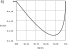
\includegraphics[width=1.0\textwidth]{Chapter_6/5}
    \caption{Примеры модулированных колебаний: а,~б)~--- по амплитуде,
    в)~--- по фазе (частоте)}
    \figmark{modulated oscillation}
\end{figure}

Будем записывать модулированные колебания в виде
\begin{equation}
    \eqmark{modulated oscillation}
    f(t)=a(t)\cos(\omega_0t+\varphi(t)).
\end{equation}
В отличие от гармонического колебания, здесь $a(t)$ и $\varphi(t)$~---
меняющиеся во времени величины. Форма записи \eqref{modulated oscillation}
особенно целесообразна в том случае, когда $a(t)$ и $\varphi(t)$~---
\important{медленно} меняющиеся функции времени, т.\,е.
эти функции остаются практически неизменными --- $a(t)\approx a_{0}$ и
$\varphi(t)\approx\varphi_0$ --- на интервалах времени~$\tau$,
существенно превышающих период гармонического (\term{несущего})
колебания частоты $\omega_0$:
\begin{equation}
    \eqmark{quasiharmonic oscillation - tau}
    \tau \gg \frac{2\pi}{\omega_0}.
\end{equation}
Такое колебание называется \term{квазигармоническим}.
В этом случае медленно меняющиеся величины~$a(t)$ и~$\varphi(t)$
принято называть \important{амплитудой} и \important{начальной фазой} модулированного колебания
соответственно.

Итак, квазигармоническое колебание можно характеризовать двумя параметрами:
периодом несущего колебания $T_0=2\pi/\omega_0$ и временем $\tau \gg T_0$,
характеризующим быстроту изменения амплитуды $a(t)$ и (или) начальной
фазы $\varphi(t)$.

Для описания модулированных колебаний используется
следующая терминология: говорят, что функция $a(t)$ описывает закон амплитудной
модуляции, а функция $\varphi(t)$~--- закон
фазовой модуляции. Именно в этих функциях и может быть заложена
передаваемая информация.

Если $\varphi(t)=\varphi_0=\const$, то
\begin{equation}
    \eqmark{amplitude-modulated}
    f(t)=a(t)\cos(\omega_0t+\varphi_0),
\end{equation}
где $a(t)\ge0$. Такое колебание называют
\term{модулированным по амплитуде}.

Если $a(t)=a_0=\const$, то
\begin{equation}
    \eqmark{phase-modulated}
    f(t)=a_0 \cos(\omega_0t+\varphi(t)).
\end{equation}
Такое колебание называют \term{модулированным по фазе}.%
\footnote{Иногда выделяют также \term{частотную модуляцию}:
    \[
     f(t)=a_0 \cos\left(\int\omega(t) dt\right).
    \]
Заменой $\omega(t) = \omega_0 + \frac{d\varphi}{dt}$ она сводится
к фазовой.}

Осциллограммы процессов на рис. \figref{modulated oscillation}а, б являются
примерами амплиту\-дно-модулированных колебаний, а на
рис.~\figref{modulated oscillation}в~--- пример колебания, модулированного по фазе.

\introsubsection{Спектры модулированных сигналов}\label{sec:modulated-spectrum}
\paragraph{Амплитудная модуляция.}
Рассмотрим простейшее амплитудно-модулированное колебание, в котором
амплитуда модуляции является гармонической функцией:
\begin{equation}
    \eqmark{example-amplitude-modulated}
    f(t)=a(t)\cos\omega_0t,\qquad \text{где~}a(t)=a_0(1+m\cos\Omega t).
\end{equation}
Константа $0<m\le 1$ называется \term{глубиной модуляции}.
Глубину модуляции можно выразить через максимальную $a_{\rm max}$ и
минимальную $a_{\rm min}$
амплитуды сигнала:
\begin{equation}
    \eqmark{modul-deep}
    m = \frac{a_{\rm max} - a_{\rm min}}{a_{\rm max} + a_{\rm min}}.
\end{equation}

Раскрывая скобки в \eqref{example-amplitude-modulated}
и пользуясь формулой для произведения косинусов, можно получить
\begin{equation}
    \centering
    \begin{aligned}
        f(t)=a_0(1+m\cos\Omega t)\cos\omega_0t=&\\
=a_0\cos\omega_0t+\frac{ma_0}{2}\cos(\omega_0+\Omega)t+
\frac{ma_0}{2}\cos&(\omega_0-\Omega)t.
    \end{aligned}
    \eqmark{ex-amplitude-modulated-sum}
\end{equation}

Итак, амплитудно-модулированное колебание с законом модуляции
\eqref{example-amplitude-modulated} представляется в виде суммы трёх
гармонических колебаний (трёх гармоник):
\begin{equation*}
    f_{0}(t)=a_0\cos\omega_0t,\quad
f_1(t)=\frac{ma_0}{2}\cos(\omega_0+\Omega)t,\quad
    f_2(t)=\frac{ma_0}{2}\cos(\omega_0-\Omega)t
\end{equation*}
с частотами соответственно $\omega_0$, $\omega_0+\Omega$, $\omega_0-\Omega$ и
амплитудами $a_0$, $ma_0/2$,
$ma_0/2$. Колебание $f_0(t)$ называется \term{несущим колебанием}, а
$f_1(t)$ и $f_2(t)$~--- \term{боковыми
гармониками}. Условие квазигармоничности колебания $f(t)$: $\Omega\ll\omega_0$.

\paragraph{Фазовая модуляция.}
Рассмотрим теперь простейший пример фазовой модуляции:
\begin{equation}
    \eqmark{example-phase-modulated}
    f(t)=a_0\cos(\omega_0t+\varphi(t)),\qquad \text{где}\quad
\varphi(t)=m\cos\Omega t.
\end{equation}
Константа $m$~--- \term{глубина модуляции фазы}~--- определяет диапазон
изменения начальной фазы (от $-m$ до $+m$).

Раскрывая косинус суммы, запишем $f(t)$ в виде
\begin{equation*}
    f(t)=a_0\bigl(\cos\omega_0t\cos\varphi(t)-\sin\omega_0t\sin\varphi(t)\bigr).
\end{equation*}

В общем случае закон модуляции \eqref{example-phase-modulated} приводит к
довольно сложному спектру (с большим числом слагаемых гармонических
колебаний). Мы рассмотрим случай $m\ll 1$ (малая глубина модуляции фазы),
когда можно использовать приближённые
выражения: $\cos\varphi(t)\approx 1$ и $\sin\varphi(t)\approx\varphi(t)$
(мы отбрасываем величины порядка $m^2$ и выше). Тогда
\begin{equation*}
    f(t)=a_0\cos\omega_0t-a_0 m\sin\omega_0t\cos\Omega t,
\end{equation*}
или (т.~к. $2\sin\alpha\cos\beta=\sin(\alpha+\beta)+\sin(\alpha-\beta)$):
\begin{multline}
    \eqmark{ex-phase-modulated-sum}
f(t)=a_0\cos\omega_0t+\frac{ma_0}{2}\cos
\left((\omega_0+\Omega)t+\frac{\pi}{2}\right)+\\
+\frac{ma_0}{2}\cos\left((\omega_0-\Omega)t+\frac{\pi}{2}\right).
\end{multline}
Это и есть искомое представление колебания $f(t)$ в виде суммы гармонических
колебаний.

\todo[inline]{Добавить на график значения боковых частот}

\begin{wrapfigure}[16]{r}{0.4\textwidth}
%     \psfragfig[width=0.5\textwidth]{Images/Chapter_6/10}{%
%     \psfrag{a}[ct]{$\omega_0$}
%     \psfrag{b}[ct]{$-\omega_0$}
%     \psfrag{c}[ct]{$\omega_0-\Omega$}
%     \psfrag{d}[ct]{$\omega_0+\Omega$}
%     \psfrag{o}[ct]{0}
%     \psfrag{1}{$a_0$}
%     \psfrag{2}{$\dfrac{ma_0}{2}$}
%     \psfrag{3}{$\dfrac{a_0}{2}$}
%     \psfrag{4}{$\dfrac{ma_0}{4}$}
%     \psfrag{x}[tl]{$\omega$}
%     \psfrag{y}{$a_n$}
%     \psfrag{z}{$c_n$}
%     \psfrag{A}{а)}
%     \psfrag{B}{б)}}
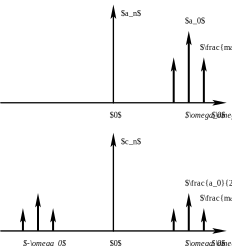
\includegraphics[width=0.4\textwidth]{Chapter_6/10}
    \caption{Спектр модулированных колебаний: действительное (вверху)
    и комплексное (внизу) представления}
    \figmark{spectrum-modulated}
\end{wrapfigure}

Сравним формулы \eqref{ex-amplitude-modulated-sum} и \eqref{ex-phase-modulated-sum}.
Первая из них~--- разложение в спектр колебания, модулированного по амплитуде,
вторая~--- колебания, модулированного по фазе. Эти колебания сильно различаются
по форме (сравните осциллограммы на рис.~\figref{modulated oscillation}б
и \figref{modulated oscillation}в), однако их спектры весьма похожи
(см. рис.~\figref{spectrum-modulated}). В обоих случаях в правой части три
слагаемых, три гармонических колебания, имеющих одинаковые частоты ($\omega_0$,
$\omega_0\pm\Omega$) и амплитуды ($a_0$~--- несущие колебания, $ma_0/2$~---
боковые гармоники). Различие выглядит небольшим: боковые гармоники отличаются
фазовым сдвигом $\frac{\pi}{2}$. Однако это различие приводит к кардинальному
отличию в форме (в осциллограмме $f(t)$) результирующего сигнала.

Приведённый пример показывает, для восстановления сигнала $f(t)$ по его спектру важно
знать \important{не только амплитуды} спектральных компонент, \important{но и их фазы}
(это важно, поскольку на практике фазы измерять сложнее, и информация о
них часто бывает утеряна).


\introsubsection{Детектирование модулированных сигналов}

Процедуру, обратную модуляции, называют \term{детектированием}.
При получении модулированного (по фазе или амплитуде) сигнала необходимо
выделить из него информацию, содержащуюся в функциях $a(t)$ или
$\varphi(t)$, отбросив по возможности высокочастотное колебание
на несущей частоте $\omega_0$ (не несущее информации).

Весь спектр модулированного сигнала сосредоточен в узкой области
вблизи большой несущей частоты $\omega_0\pm \Omega$, где $\Omega$ ---
характерная частота модуляции. Необходимо преобразовать сигнал так,
чтобы полезная информация оказалась в области низких частот. Это можно
сделать \important{нелинейными} элементами. Одним из простейших способов
детектирования является использование элементов с квадратичным законом связи
(\term{квадратичное детектирование}) между входным и выходным сигналом:
$g(t)\propto f^2(t)$ (другой способ --- использование \term{выпрямляющих}
преобразователей, например, полупроводниковых диодов).

Для того, чтобы избавиться от <<ненужных>> (не содержащих полезную
информацию) высокочастотных составляющих можно применять обычные линейные
фильтры (см., в частности, Пример~\ref{exmpl:RC}). Действие такого фильтра может быть сведено к усреднению во времени
сигнала по интервалу $\Delta t$, который существенно превосходит период
колебаний несущей, но значительно меньше периода колебаний <<информативных>>
функций $a(t)$ или $\varphi(t)$:
\begin{equation}
    \eqmark{averages-sq}
g(t) = \left<f^2(t)\right>_{\Delta t} = \frac{1}{\Delta t}
\int\limits_{t}^{t+\Delta t} f^2(t')\,dt',
\end{equation}
где
\begin{equation}
    \eqmark{averages-cond}
    \frac{2\pi}{\omega_0} \ll \Delta t \ll \frac{2\pi}{\Omega}.
\end{equation}
Схема квадратичного детектирования приведена на рис.~\figref{detect2}.
\begin{figure}[h]
 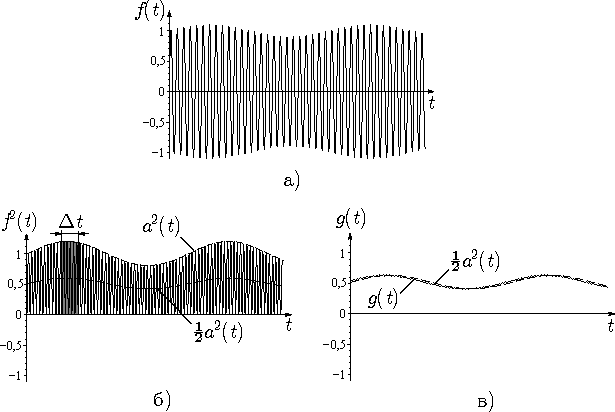
\includegraphics[width=\textwidth]{Chapter_6/v6-detect2.pdf}
 \caption{Схема детектирования модулированного сигнала:
     а) исходный сигнал $f(t)$, б) квадратичный сигнал
 $f^2(t)$, в) результат $g(t)$ усреднения по интервалу $\Delta t$.
Отличие $g(t)$ от $\frac12a^2(t)$ (отклонение и шум)
связаны с недостаточно хорошим выполнением сильного неравенства
\eqref{averages-cond}}
 \figmark{detect2}
\end{figure}

\paragraph{Квадратичное детектирование амплитудно-модулированного сигнала.}
Рассмотрим, как преобразование \eqref{averages-sq} действует на
амплитудно модулированный сигнал $f(t) = a(t) \cos \omega_0 t$. Имеем
\[
 g(t) = \left<f^2(t)\right>_{\Delta t} =
 \frac{1}{\Delta t}
\int\limits_{t}^{t+\Delta t} a^2 (t') \cos^2(\omega_0 t')\,dt'.
\]
Ввиду соотношения \eqref{averages-cond} амплитуда~$a(t)$ практически не меняется
на отрезке $[t,\,t+\Delta t]$, поэтому её можно вынести из-под знака интеграла:
\begin{equation}
 g(t)= \frac{a^2(t)}{\Delta t} \int\limits_{t}^{t+\Delta t} \cos^2(\omega_0 t')\,dt'\approx
 \frac12 a^2(t).
\end{equation}
Последний переход справедлив, поскольку $\Delta t \gg 2\pi/\omega_0$ и
можно приближённо считать, что интегрирование ведётся по целому числу периодов
$2\pi /\omega_0$.
Таким образом, предложенная схема измеряет \important{квадрат амплитуды модуляции}.

Если имеет место модуляция гармонической функцией
\eqref{example-amplitude-modulated}
с малой глубиной модуляции $m\ll 1$, то
\[
 g(t) = \frac12 a_0^2 (1+m\cos\Omega t)^2 \approx
 \frac12 a_0^2 (1+2m\cos\Omega t).
\]
Видно, что после квадратичного детектирования остаётся гармонический
сигнал $m a_0^2 \cos\Omega t$ на частоте модуляции, существующий на фоне
постоянного сигнала $a_0^2/2$.

\paragraph{Квадратичное детектирование фазово-модулированного сигнала.}
У сигнала, модулированного по фазе, амплитуда постоянна: $a(t)=\const$.
Можно ли в таком случае использовать квадратичное детектирование?

Как мы выяснили выше, спектры фазово- и амплитудно-модулированного сигналов
отличаются лишь начальными фазами гармоник. Изменив с помощью линейного фильтра
фазу несущего колебания (или боковых гармоник) на $\frac{\pi}{2}$,
мы можем преобразовать колебание, модулированное по фазе,
в амплитудно-модулированное колебание. Это известный в
радиотехнике \term{приём с изменением фазы несущей}.

Ещё один один метод --- \term{приём без несущей}, при котором из
спектра <<убирается>> (также линейным фильтром)
несущее колебание $a_0\cos\omega_0t$. Предлагаем читателю самостоятельно
проанализировать, что будет представлять собой результирующее колебание.

Аналогичные приёмы преобразования фазовой модуляции в амплитудную
применяются в оптике при наблюдении прозрачых структур ---
методы <<фазового контраста>> и <<тёмного поля>>.


\introsection{Синтез сигналов}\label{sec:synth}

Возможность разложить произвольную функцию $f(t)$ в ряд (или интеграл)
Фурье единственным и однозначным способом подразумевает и возможность
<<собрать>> сигнал любой формы, используя гармонические колебания с подобранными
амплитудами и фазами, совершив таким образом \important{обратное} преобразование Фурье.

Спектр реального сигнала в общем случае содержит бесконечное количество
гармоник, поэтому синтезировать исходный сигнал можно, как правило,
лишь в некотором приближении. Степень совпадения будет определяться
количеством синтезирующих гармоник (чем больше, тем лучше).

\begin{figure}[h!]
 \centering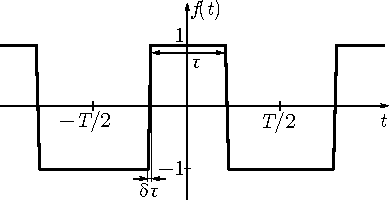
\includegraphics[scale=0.9]{Chapter_6/v6-meandr.pdf}
 \caption{Прямоугольный сигнал (меандр)}
 \figmark{meandr-delta}
\end{figure}

Рассмотрим в качестве примера прямоугольный сигнал, принимающий
значения $\pm 1$ со скважностью $\tau/T=1/2$ (<<меандр>>,
рис.~\figref{meandr-delta}). Из формулы \eqref{impulses-spectrum} имеем спектр
\[
c_n = \frac{\sin \pi n/2}{\pi n/2}.
% =
% \begin{cases}
%     0 & n\text{~--- чётное},\\
%     \frac{(-1)^{\frac{n-1}{2}}}{\pi n}& n\text{~--- нечётное}.
% \end{cases}
\]
Переходя к амплитудам и фазам согласно \eqref{Fourier-coefficient},
найдём
\[
a_{2k}=0,\quad a_{2k-1} = \frac{4}{\pi (2k-1)},\quad
\varphi_{2k-1} = \pi (k-1),\qquad k=1,\,2,\,\ldots
\]
($c_0=a_0=0$). Первые несколько слагаемых в спектральном разложении:
\[
f(t) \approx \frac{4}{\pi} \left[ \cos \omega_0 t -
\frac{1}{3}\cos 3\omega_0 t +
\frac{1}{5}\cos 5\omega_0 t -
\frac{1}{7}\cos 7\omega_0 t + \ldots\right]
\]
На рис.~\figref{meandr-synthesis} представлен результат аппроксимации
рассматриваемой функции $k$ первыми слагаемыми её ряда Фурье.
Видно, что с увеличением числа слагаемых аппроксимация становится всё точнее.

При внимательном рассмотрении можно заметить интересную особенность:
колебания частичной суммы ряда особенно сильны около точек разрыва
функции $f(t)$. Причём
амплитуда первого максимума этих колебаний (в непосредственной близости от
разрыва) \important{не убывает} с ростом числа слагаемых (и составляет около 18\%
от величины скачка). Это явление получило название \term{явление Гиббса}.
Математически оно является следствием \important{неравномерной} сходимости ряда
Фурье разрывной функции. Если функция непрерывна и ограничена, то сходимость
её ряда Фурье будет равномерной (\important{признак Дирихле}) и подобных проблем
не возникает\footnote{См., например,
\important{Фихтенгольц Г.М.} Курс дифференциального и интегрального исчисления,
Т.~III, Гл.~19, \S4.}.

\begin{figure}[h!]
 \hfill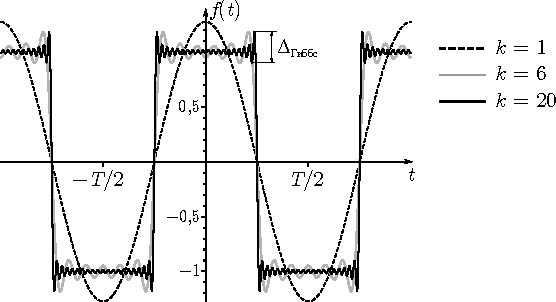
\includegraphics{Chapter_6/v6-synthes.pdf}
 \caption{Аппроксимация разрывной функции частичными суммами ряда Фурье
 ($k$ --- число ненулевых слагаемых)}
\figmark{meandr-synthesis}
\end{figure}

С физической точки зрения по-настоящему \important{мгновенный} скачок функции
невозможен~--- всегда есть какое-то конечное (возможно, очень малое) время
перехода~$\delta\tau$. В таком случае явление Гиббса исчезнет, когда в
частичную сумму ряда Фурье попадут слагаемые, с помощью которых можно
<<разрешить>> столь малые масштабы по времени, то есть с частотами
порядка $\omega \sim 2\pi /\delta \tau$.

\begin{lab:questions}
\item Как можно измерить коэффициенты ряда Фурье (спектр) некоторого сигнала?

\item Изобразите схематично спектры $C(\omega)$:
\begin{itemize}
    \item бесконечно длинной синусоиды;
    \item синусоиды конечной длины;
    \item периодической последовательности прямоугольных импульсов;
    \item одного прямоугольного импульса.
    \item периодической последовательности цугов;
    \item одного цуга.
\end{itemize}

\item Чем отличаются спектры амплитудно- и фазово-модулированного сигналов?

\item Как изменится спектр периодической последовательности
прямоугольных импульсов, если убрать каждый второй импульс?

\item Как изменится спектр периодической последовательности прямоугольных
импульсов, если уменьшить длительность каждого импульса в два раза?

\item Что такое детектирование? Какие существуют методы детектирования
фазово-модулированного сигнала?

\item Предложите электрическую схему низкочастотного линейного фильтра.

\item Периодический прямоугольный сигнал подали на интегрирующую $RC$-цепочку
(рис.~\figref{RC}). Как в результате изменится форма сигнала?

\end{lab:questions}

\begin{lab:literature}
    \item \textit{Сивухин~Д.В.} Общий курс физики.~Т.III. Электричество ---
М.:~Физматлит, 2003.~--- \S~128.
    \item \textit{Кингсеп~А.С., Локшин~Г.Р., Ольхов~О.А.} Основы физики.~Т.I.---
М.:~Физматлит, 2007.~--- Гл I, \S\S~1.5, 1.6.
    \item \textit{Кириченко Н.А.} Электричество и магнетизм: учебн. пособие.---
    М.:~МФТИ, 2011.~--- \S\S~17.4--17.7.
    \item \textit{Локшин~Г.Р., Козел~С.М.} Модулированные колебания. Спектральный
анализ. Линейная фильтрация --- М.:~МФТИ, 2009.
\item *\textit{Булыгин В.С.} Явление Гиббса --- М.:~МФТИ, 2014.
\end{lab:literature}

% ---------------------------------------------



